\documentclass[PhD-Yoann-Dupont.tex]{subfiles}
\begin{document}

Les CNN sont des réseaux de neurones dont le principe est d'observer localement l'espace d'entrée afin de déterminer la sortie à une position donnée. Dans le traitement de l'image, cela revient à en observer une zone plutôt qu'un pixel. Pour le traitement d'une séquence, cela équivaut à utiliser une fenêtre coulissante observant l'élément courant ainsi que son contexte immédiat jusqu'à une distance donnée. Typiquement, cette fenêtre considère que le token courant se situe au milieu, auquel cas le calcul d'une telle couche se fait de la façon suivante :

\begin{equation}\label{eq:CNN-formula}
cnn(x)_{i} = W_{cnn} \times \left[ x_{i-\lceil l/2 \rceil} ... x_{i} ... x_{i+ \lfloor l/2 \rfloor} \right]\\ pour\ 1+\lfloor l/2 \rfloor \leq i \leq (s - \lfloor (l-1)/2 \rfloor)
\end{equation}

Où les crochets $[\ ]$ représentent l'opération de concaténation, $\lceil x \rceil$ est l'arrondi à l'entier supérieur, $\lfloor x \rfloor$ l'arrondi à l'entier inférieur, $W_{cnn}$ est la matrice de paramètres du CNN ajustée à l'apprentissage et l la taille de la fenêtre coulissante et s la taille de la séquence. Ces opérations sont exemplifiés sur la figure \ref{fig:CNN-detail}.

Sur l'exemple donné dans la figure \ref{fig:CNN-detail}, la couche de convolution peut se voir comme une fenêtre coulissante de taille 3, observant le token courant ainsi que son contexte gauche et droit à une distance de 1, le détail d'une telle convolution étant donné dans la figure \ref{fig:CNN-detail}. Un CNN permet de fournir une représentation dense d'un token dans le contexte local dans lequel il apparaît. Cette information est plus intéressante que la simple concaténation des différents tokens,

\begin{figure}[ht!]
    \centering
    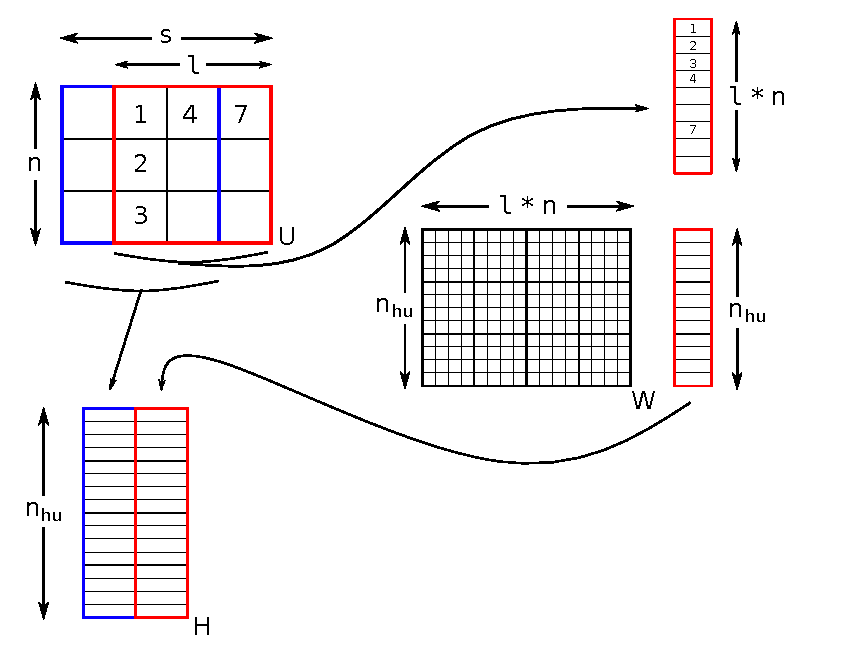
\includegraphics[scale=0.8]{images/NN/convnet}
    \caption{détail des opérations effectuées pour une convolution temporelle. $U$ est la séquence en entrée, $W$ est la matrice de paramètres et $H$ est la séquence en sortie. $n$ est la taille des représentations, $s$ la taille de la séquence, $l$ la taille de la fenêtre, $n_{hu}$ la taille de la couche cachée. Pour chaque fenêtre de taille $l$, les $l$ vecteurs de $U$ sont concaténés et multipliés à la matrice de paramètre $W$ pour donner un élément de la séquence de sortie $H$. Nous pouvons voir que le nombre d'éléments de $H$ est inférieur à celui de l'entrée. Cette réduction de dimensionalité impose à utiliser du padding afin de conserver une taille cohérente par rapport au nombre de tokens de U.}
    \label{fig:CNN-detail}
\end{figure}

\citet{collobert2008unified} propose une approche afin d'utiliser les CNN dans le domaine du TAL, pour des tâches d'étiquetage de séquences et de classification de phrases, dont le principe général est illustré dans la figure \ref{fig:CNN-collobert2008}. Cette méthode a été utilisée sur de nombreuses tâches où elle était proche de l'état-de-l'art voire état-de-l'art.

\begin{figure}[ht!]
\centering
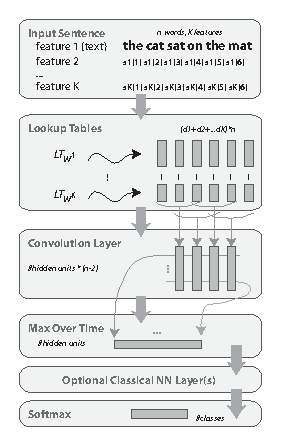
\includegraphics[scale=1.25]{images/general/collobert2008}
\caption{un réseau de neurones à convolution de \citet{collobert2008unified}}
\label{fig:CNN-collobert2008}
\end{figure}

Un CNN étant un FFNN, il souffre donc des inconvénients de ces derniers. Pour l'annotation de séquences, les réseaux de neurones récurrents sont privilégiés, en particuliers les LSTM, que nous détaillerons dans la section suivante.

\end{document}